
\documentclass[11pt]{article}
\usepackage[margin=0.9in]{geometry}
\usepackage{graphicx,amsmath,booktabs}
\title{Shifting an inner circle:\\angular dipole on its surface}
\author{}
\date{}
\begin{document}
\maketitle
\noindent Simple geometry only. Outer circle radius $R=2r$; inner circle radius $r$ shifted by $r/2$. Guides show how equal chunks of the outer circle map onto the inner surface. No cosmology labels.

\begin{center}
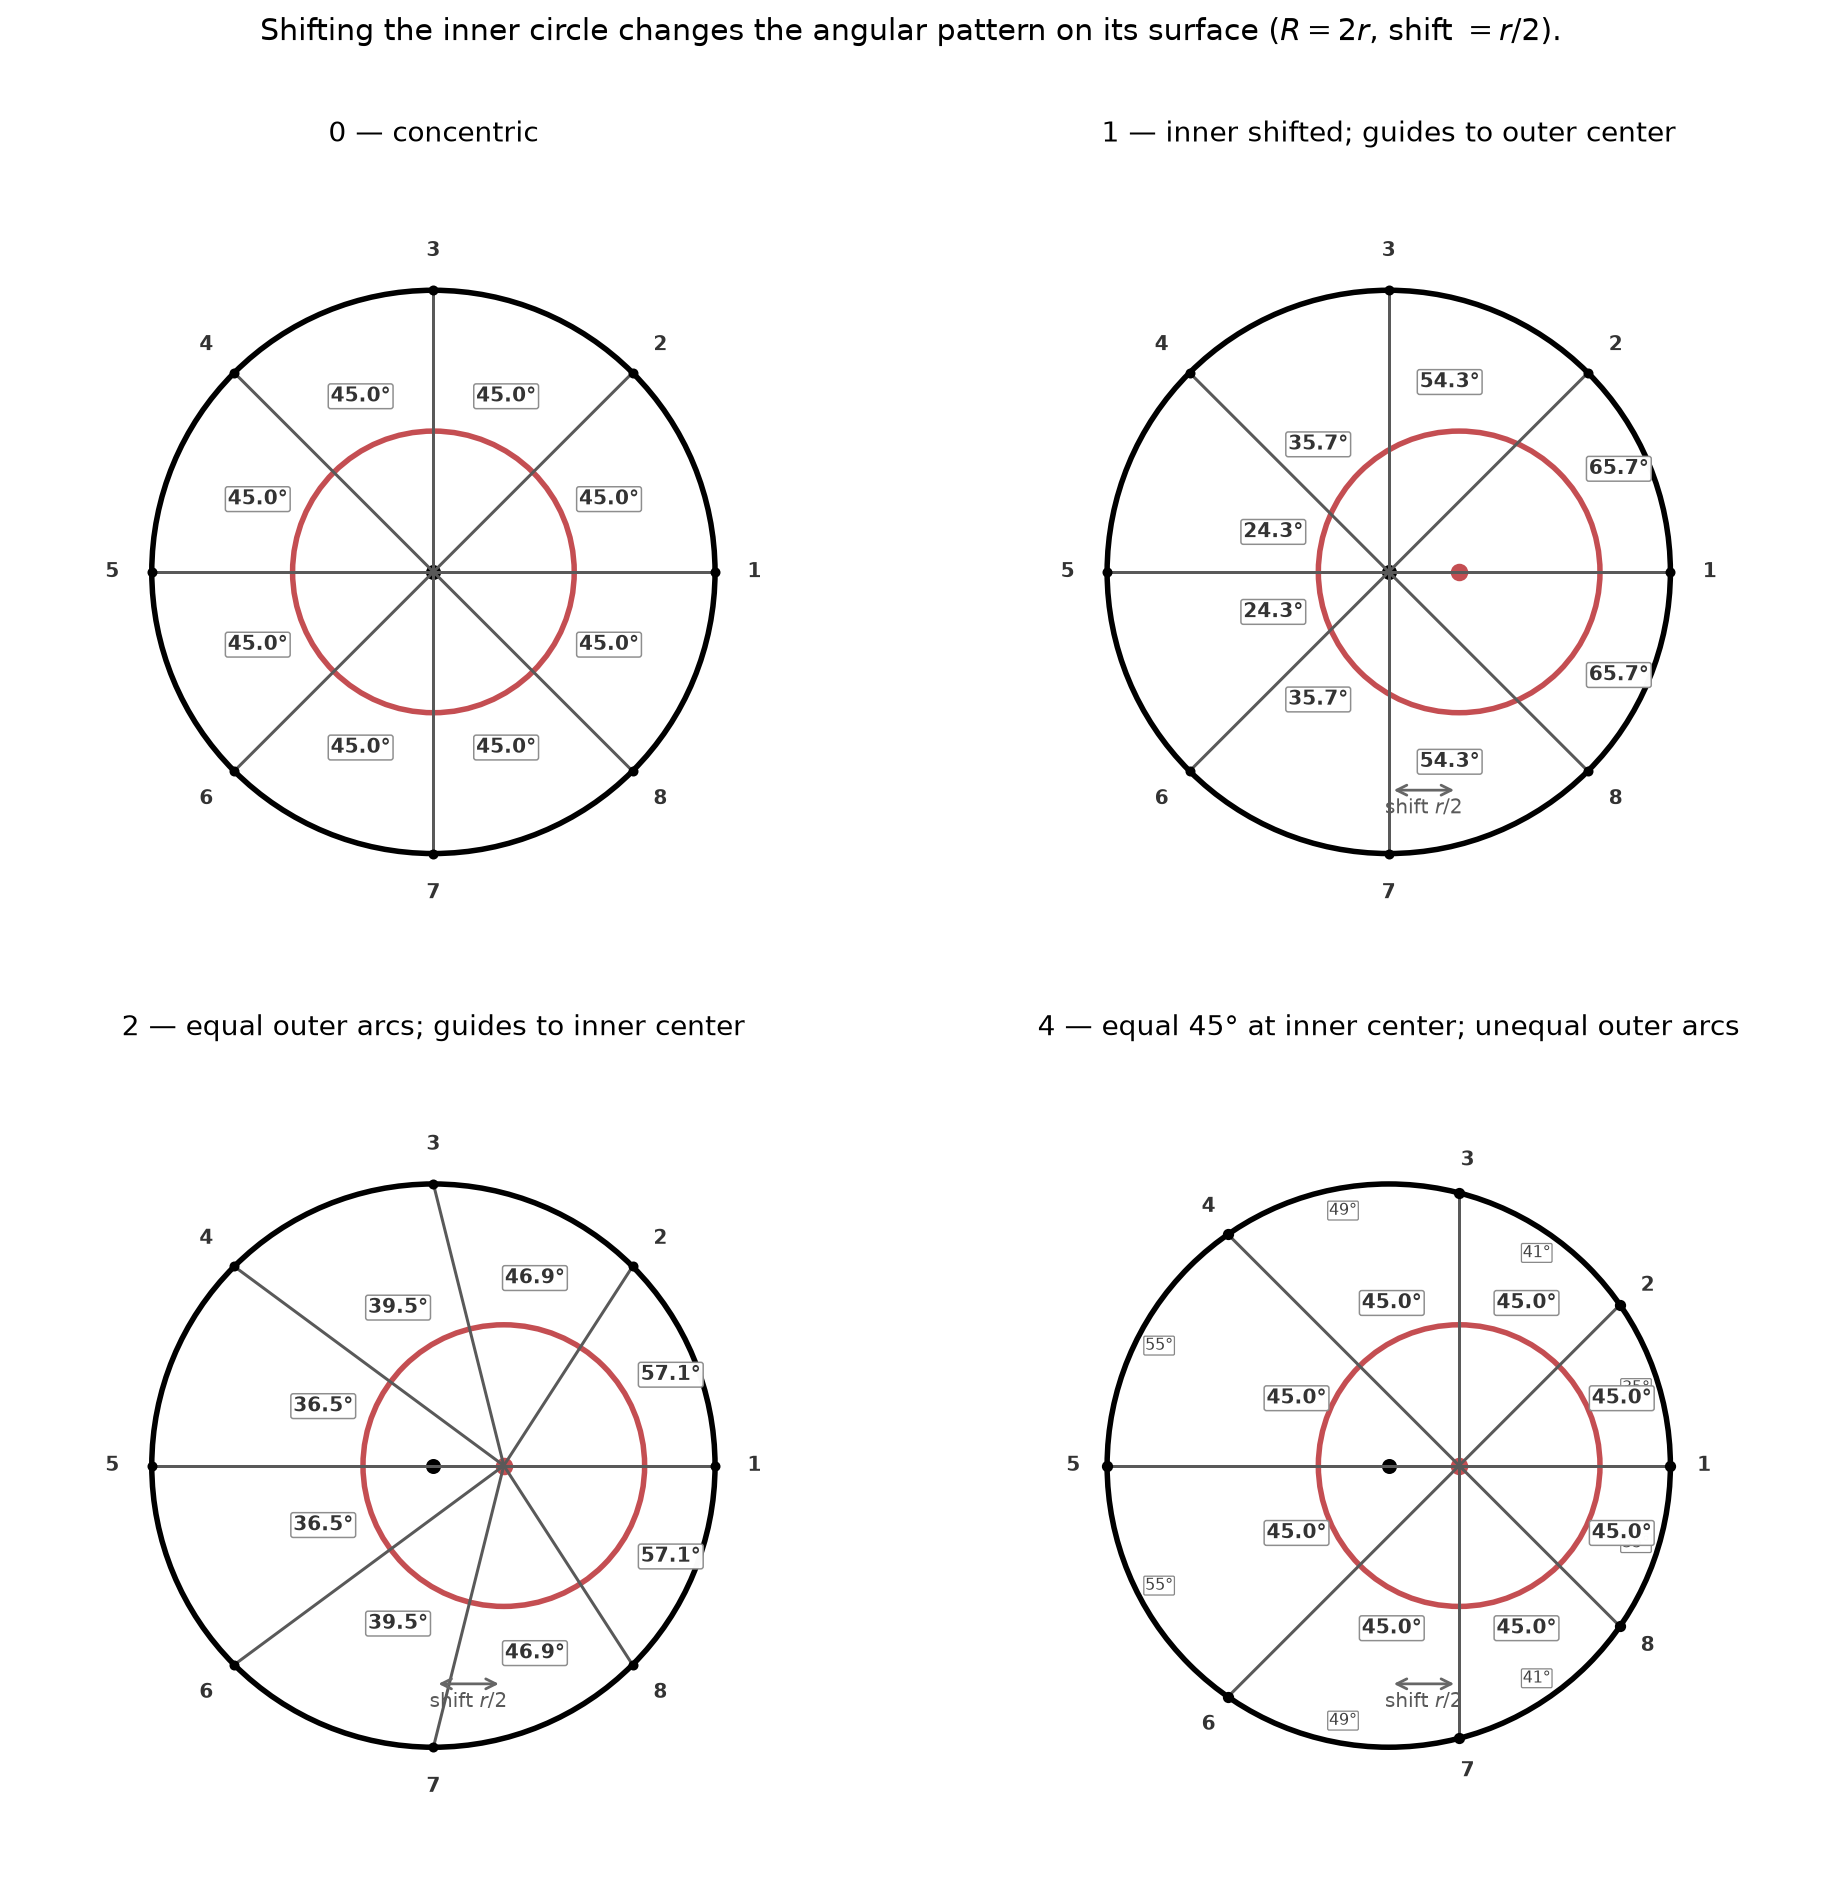
\includegraphics[width=\textwidth]{figures/four_scenarios_overview.png}
\end{center}

\section*{Scenarios}
\begin{itemize}
\item \textbf{0} Concentric: equal angles all around (all $45^\circ$).
\item \textbf{1} Inner shifted; guides still through the outer center: angles on the inner surface are unequal.
\item \textbf{2} Equal outer arcs, guides to the inner center: unequal angles on the inner surface.
\item \textbf{4} Equal $45^\circ$ at the inner center: each wedge takes a different outer arc length.
\end{itemize}

Shifting the inner circle produces an angular dipole pattern on its surface (crowding on the side toward the outer center).

\end{document}
